\documentclass[a4paper,12pt]{report}
\usepackage[utf8]{inputenc}
\usepackage[T1]{fontenc}
\usepackage[italian]{babel}
\usepackage{amsmath}
\usepackage{listings}
\usepackage{amssymb}
\usepackage{cancel}
\usepackage{tikz}
\usetikzlibrary{angles, quotes}
\usepackage{tikz-3dplot}
\usepackage{mathptmx}
\usepackage{tzplot}
\newcommand{\taninv}{\tan^{-1}}
\usepackage{titlesec}
\usepackage{multicol}
\usepackage[only,llbracket,rrbracket]{stmaryrd}
\newcommand\val[1]{\llbracket#1\rrbracket}
\newcommand\Iff{\Leftrightarrow}
\newcommand\raa{RAA}
\usepackage{graphicx}

\graphicspath{{./img/}}


\newcommand\qed{\begin{flushright}{$\square$}\end{flushright}}


\titleformat{\chapter}
	{\Large\bfseries}		% format
	{}							% label
	{0pt}						% sep
	{\huge}					% before-code

\begin{document}
\title{Appunti del corso di Logica 

A.A. 2023/2024}
\author{Note a cura di Niccol\`{o} Iselle\\
Corso della Prof. Alessandra Di Pierro}
\date{}
\maketitle
\tableofcontents

\chapter{Introduzione}
% ============================= LEZIONE 1 - 2/10/23 =============================
\section{Logica - `Studio del ragionamento'}
Possiamo suddividere la \emph{logica} in due categorie: quella \emph{formale}, ovvero \emph{simbolica}, che \`{e} lo sudio dei passaggi del nostro ragionamento basati su connettivi nelle nostre `sentenze' (\emph{if, and, or}); e quella \emph{informale} (non simbolica), che \`{e} lo studio del pensiero logico in un contesto informale come la critica o l'argomentazione, pi\`{u} inerente al campo filosofico. 

\section{`La barretta di cioccolata'}
Consideriamo una barretta di cioccolata formata da 24 quadratini disposti in un
rettangolo 6 x 4. Il nostro obbiettivo \`{e} quello di separare ogni quadratino
col minor numero di tagli (sempre effettuati lungo le linee). Quanti tagli serviranno?

\paragraph{Soluzione:} intuitivamente serviranno tanti tagli quanti sono i quadratini di cioccolata meno uno.

\subsection{Dimostrazione per induzione}
\paragraph{Principio di induzione:} 
\begin{itemize}
\item $ P(n) $
\item $ P(0) $
\item $ P(n-1) $ ipotesi induttiva, se assumendo che $P$ \`{e} vera su $n-1$.
\item Dimostriamo che $P(n)$, allora $P$ vale per ogni $n$.
\end{itemize}
\paragraph{Dimostrazione:}

\begin{enumerate}
\item Se la barretta \`{e} fatta da un quadratino $\rightarrow$ banale, 0 tagli.
\item Assumendo che per una barretta composta da $1 < m < N$ quadratini abbiamo gi\`{a} dimostrato che servono esattamente $m - 1$ tagli per una barretta composta da $m$ quadratini. 
\item Se ora abbiamo una barretta da $N$ quadratini, e la dividiamo in due parti $m_1$ ed $m_2$. Ovviamente $m_1 + m_2 = N$. Per l'ipotesi induttiva, ci serviranno $m_1 - 1$ tagli per separare i quadratini di $m_1$ ed $m_2 - 1$ tagli per separare i quadratini di $m_2$. Il totale sar\`{a} quindi \[1 + (m_1 - 1) + (m_2 -1) = N - 1\]
\end{enumerate}

\subsection{Dimostrazione per invariante}
\paragraph{Invariante:} si tratta di una propriet\`{a} che non cambia il suo valore, ovvero una proposizione \emph{vera}. Ad esempio, in un programma l'invariante \`{e} quella propriet\`{a} che rimane uguale prima, durante e dopo l'esecuzione del programma stesso.
\newline

Per dimostrare che servono $N-1$ tagli per separare la barretta di cioccolata nei singoli quadratini. Possiamo notare che ogni volta che rompiamo la barretta il numero totale di pezzi aumenta di uno (il pezzo pi\`{u} grande viene diviso in due pezzi pi\`{u} piccoli). Quando non abbiamo pi\`{u} pezzi da rompere, ogni pezzo \`{e} un quadratino. All'inizio, dopo 0 tagli, abbiamo 1 pezzo. Dopo aver fatto 1 taglio, otteniamo 2 pezzi. Aumentare il numero dei tagli di 1 fa aumentare il numero di pezzi di 1. Quindi il secondo numero (numero di quadratini) sar\`{a} sempre di 1 pi\`{u} grande del primo (numero di tagli).

\section{Concetto di insieme}

Possiamo definire un insieme in modo estensivo
\[ A = \{a, b, c\} \]
elencando tutti i suoi elementi, oppure possiamo definirlo utilizzando una propriet\`{a} condivisa da tutti i suoi elementi
\[ A = \{x | x \text{ \`{e} pari}\} \subseteq \mathbb{N} \]
che equivale a scrivere
\[ \{x | x \in \mathbb{N} \text{ e $x$ \`{e} pari}\} \]
o ancora
\[ \{x \in \mathbb{N} | x \text{ \`{e} pari}\} \]

\section{Logica proposizionale (o sentenziale)}

La logica proposizionale \`{e} un ramo della logica simbolica deduttiva che assume le proposizioni (sentenze) come unit\`{a} fondamentali dell'analisi logica. Le preposizioni che prendiamo in esame sono le \emph{asserzioni}.

\paragraph{Asserzione:} \`{e} una proposizione che ha un valore di verit\`{a}, cio\`{e} pu\`{o} assumere il valore \emph{vero (T)} oppure il valore \emph{falso (F)}.

\paragraph{Esempi di asserzioni:}
\begin{itemize}
\item Verona \`{e} una citt\`{a} del Veneto
\item Fuori sta piovendo
\item Nel 5024 il Sole si spegner\`{a}
\end{itemize}

Le asserzioni possono essere collegate da \emph{connettivi logici} tra loro. Prendiamo in esempio la frase `\emph{Se \underline{c'\`{e} il sole} allora \underline{serve la protezione}. Ma se \underline{serve la protezione} allora
\underline{non si pu\`{o} fare il bagno}.}'
Possiamo estrapolare tre asserzioni:
\begin{itemize}
\item S: \emph{C'\`{e} il sole}
\item P: \emph{Serve la protezione}
\item B: \emph{Non si pu\`{o} fare il bagno}
\end{itemize}
e possiamo collegarle tra loro con i connettivi logici, per formare lo stesso significato espresso dalla frase, nel modo in cui segue:
\[ S \rightarrow P \]
\[ P \rightarrow B \]
(Dove $\rightarrow$ si legge \emph{implica}).

\subsection{Linguaggi formali - (automi di riconoscimento)}

Nella logica dobbiamo usare un linguaggio formale, formato da un \emph{alfabeto}. Un esempio di definizione di alfabeto potrebbe essere il seguente:
\[ A = \{a, b\} \]
Un linguaggio formale, basato sull'alfabeto $A$ potrebbe essere:
\[ L(A) = \{a, b, ab, aa, ba, \dots \} \]
Notare che $ab \ne ba$, si dice che sono \emph{parole} diverse.
Un'altra notazione importante \`{e} \emph{A-star} scritta come $A^{*}$, che sta ad indicare tutte le stringhe che si possono costruire con l'alfabeto A.
\paragraph{Esempio:}

Dato l'alfabeto $A = \{a, b\}$, costruiamo un linguaggio costituito da tutte le stringhe formate da un numero pari di simboli:
\[ L_p = \{aa, ab, abab, \dots\} \]
Possiamo quindi affermare che $a \notin L_p$.


\section{Teoria dell'Aritmetica di Peano - Definizione dei numeri naturali}

Per definire i numeri naturali, utilizziamo una \emph{struttura} formata da tre elementi:
\[ <\mathbb{N}, 0, succ> \]
\begin{itemize}
\item $\mathbb{N}$ \`{e} l'universo del discorso
\item $0$ \`{e} una costante, il caso base
\item $succ$ \`{e} una funzione su $\mathbb{N}$ definita come \[ succ: \mathbb{N} \rightarrow \mathbb{N} \]
\end{itemize}

\subsection{I ASSIOMA}

\begin{center} Esiste un numero $0 \in \mathbb{N}$ \end{center}
Il primo assioma dice che $0$ \`{e} un elemento privilegiato di $\mathbb{N}$ detto \emph{zero}.

\subsection{II ASSIOMA}
\begin{center} Esiste una funzione $succ:  \mathbb{N} \rightarrow \mathbb{N}$ \end{center}

Il secondo assioma dice che $succ$ \`{e} un'operazione unaria iniettiva su A;

\subsection{III ASSIOMA}
\[ succ(x) \ne 0 \text{ per ogni } x \in \mathbb{N} \]
Il terzo assioma ci dice che 0 non \`{e} il successore di nessun numero, un altro modo di esprimerlo \`{e} $0 \notin Im(succ)$.

\subsection{IV ASSIOMA}
\begin{center} Se $P \subseteq \mathbb{N}$ e valgono le seguenti propriet\`{a}:
\begin{itemize}
\item $0 \in P$
\item $\forall n \in \mathbb{N}.(n \in P \rightarrow succ(n) \in P)$,
\end{itemize}
allora $P = \mathbb{N}$.
\end{center}
Il quarto assioma sta ad indicare che, partendo dal fatto che 0 \`{e} un numero naturale, se $n$ \`{e} un numero naturale allora anche $n+1$ \`{e} un numero naturale. Questo assioma \`{e} detto \emph{assioma di induzione}.

\section{Principio di Induzione}
Dato che una propriet\`{a} $P$ sui numeri naturali non \`{e} altro che un sottoinsieme di $\mathbb{N}$, ovvero $P\subseteq\mathbb{N}$, possiamo riformulare l'assioma di induzione come principio per provare propriet\`{a} sui naturali.
\subsection{Principio di induzione:}
Sia $P(x)$ una propriet\`{a} su $\mathbb{N}$. \newline
Se $P(0)$ e $\forall n \in \mathbb{N}.(P(n) \rightarrow P(succ(n))$ allora $\forall m \in \mathbb{N}.P(m)$.

\subsection{Esempio}
Dimostrare per induzione su $n$ che 
\[ P(n) \equiv \sum_{i=0}^{n}2i+1 = (n+1)^2 \]

\paragraph{Caso base $n=0$:}
\[ \sum_{i=0}^{0} 2i+1 = (n+1)^2 \]
\[ 2*0+1 = (0 + 1)^2 = 1 \]

\paragraph{Ipotesi induttiva:} supponiamo ora che valga 
\[ \sum_{i=0}^{n-1} 2i+1 = ((n-1)+1)^2 \]
e utilizziamo questa \emph{ipotesi induttiva} per dimostrare che vale anche per $n$.

\paragraph{Passo induttivo:}

Partiamo dalla formula che dobbiamo dimostrare 
\[ \sum_{i=0}^{n}2i+1 = (n+1)^2 \]
e possiamo riscriverla come
\[ \sum_{i=0}^{n-1} 2i+1 + 2n+1 = (n+1)^2 \]
ora possiamo utilizzare l'ipotesi induttiva, sapendo che 
\[ ((n-1)+1)^2 + 2n+1 = n^2 + 2n + 1 \]
e risolviamo:
\[ (n-1)^2 + 2(n-1) + 1 + 2n + 1 = n^2+2n+1 \] 
\[ n^2-2n+1+2n-2+1+2n+1 = n^2+2n+1 \]
\[ n^2+2n+1 = n^2+2n+1 \]
\begin{flushright}{$\square$}\end{flushright}


% ============================= LEZIONE 2 - 5/10/23 =============================
\section{Cardinalit\`{a} di un insieme}
La cardinalit\`{a} di un insieme \`{e} il numero di elementi che esso contiene, per esempio:
\[ \mathbb{N} = \{ 1, 2, 3, \dots \} \]
La cardinalit\`{a} di $\mathbb{N}$, che si esprime in notazione come $|\mathbb{N}|$ \`{e} un \emph{infinito numerabile}.
Nel caso di un insieme con un numero finito di elementi, ad esempio $A = \{a, b, c \}$ la sua cardinalit\`{a} $|A| = 3$.

Se un insieme ha la stessa cardinalit\`{a} di $\mathbb{N}$ significa che pu\`{o} essere messo in \emph{corrispondenza biunivoca} con $\mathbb{N}$.
Ovvero 
\[ \forall b\in B \exists n \in \mathbb{N} \]
\[ f: b \rightarrow n \]
E vale anche che
\[ \forall b \in \mathbb{N} \exists b \in B \]
\[ f: n \rightarrow b \]

\section{Numeri naturali}
Come precedentemente detto, i numeri naturali sono formati da
\[ \left<\mathbb{N}, succ, 0\right> \]
$succ: \mathbb{N} \rightarrow \mathbb{N}$ \`{e} una funzione \emph{iniettiva}, ovvero ad ogni elemento del dominio corrisponde uno e uno solo elemento dell'immagine. 
Presi due insiemi $A$ e $B$, se $Im(f) = B$ si dice che la funzione \`{e} \emph{surgettiva}. 
Se una funzione \`{e} \emph{surgettiva} e \emph{iniettiva} si ha una \emph{corrispondenza biunivoca (biezione)}.
\subsubsection{Esempio di proposizione sui numeri naturali}
\[P:= n \text{ \`{e} pari} \]
\[ P = {n \in \mathbb{N} | P(n) } \]
\[ = {n \in \mathbb{N} | n \text{ \`{e} pari}} \] 

\subsection{Definizioni induttive}

\subsubsection{Esempio}
Definiamo $h$ come segue
\[ h: \mathbb{N}x\mathbb{N} \rightarrow \mathbb{N}\thickspace \text{ t.c. }  h(x,y) = succ(x) * y \]

\paragraph{caso base} \[f(0) = 1 \]
\[f(succ(n) = h(n, f(n)) = succ(n) * f(n) \]

\paragraph{n = 0}
\[ succ(0) * f(0) = 1 * 1 = 1 \]

\paragraph{caso induttivo}
\[ f(succ(succ(0))) = succ(n) * f(n) \]

\paragraph{n = 2}
\[ f(succ(succ(0)) = f(2) = 2 * 1 = 2 \]
\paragraph{n = 3}
\[ f(succ(succ(succ(0)))) = f(3) = 3 * 2 * 1 \]
\[ \dots \]
Possiamo notare che questa \`{e} la definizione induttiva del fattoriale di un numero.
\chapter{Sintassi}
\section{Simboli e significato}
\begin{tabular}{| c | c |}
\hline
\textbf{Simboli} & \textbf{Significato} \\ 
\hline
$P \to Q$ & \emph{se} P \emph{allora} Q \\
\hline
$P \leftrightarrow Q$ & P \emph{se e solo se} (\emph{sse}) Q \\
\hline
$P \wedge Q$ & P \emph{and}/\emph{e} Q \\
\hline
$P \lor Q$ & P \emph{or}/\emph{oppure} Q \\
\hline
$\neg P$ & \emph{not} P (P \`{e} \emph{falso}) ($(\neg P) \equiv (P \to \bot)$) \\
\hline
$\forall x P$ & \emph{per ogni elemento x P(x) \`{e} vero} \\
\hline
$\exists x P$ & \emph{Esiste un elemento tale che P \`{e} vero per quell'elemento} \\
\hline
\end{tabular}

% ============================= LEZIONE 3 - 9/10/23 =============================
\section{Linguaggio formale}
Il linguaggio della logica proposizionale ha un alfabeto che consiste di 
\begin{enumerate} 
\item proposizioni (o simboli proposizionali): $p_0, p_1, p_2, \dots$
\item connettivi: $\wedge, \lor, \to, \leftrightarrow, \neg, \bot, \top$
\item simboli ausiliari: `(` e `)'
\end{enumerate}

\subsubsection{Bottom e Top}
\begin{itemize}
\item Bottom \`{e} il falso e si indica con $\bot$, il suo valore \`{e} sempre 0.
\item Top \`{e} il vero e si indica con $\top$, il suo valore \`{e} sempre 1 e viene definito come $\vDash \top \leftrightarrow (\bot \to \bot)$.
\end{itemize}

\subsection{Proposizioni atomiche e proposizioni composte}
\subsubsection{Proposizioni atomiche o minimali}
Le proposizioni atomiche sono quelle proposizioni che non possono essere suddivise in parti pi\`{u} piccole. Per esempio \[ 5 \in \{0, 1, 2, 3, 4, 5\} \]
\`{e} una proposizione atomica.

\subsubsection{Proposizioni composte} 
\[ c \text{ \`{e} razionale oppure $c$ \`{e} irrazionale} \]
Una proposizione si dice composta quando pu\`{o} essere scomposta in sotto-proposizioni pi\`{u} piccole, unite da connettivi logici ($\wedge, \lor, \to, \dots $).

\subsection{L'insieme $PROP$ delle proposizioni}
L'insieme $PROP$ \`{e} il \emph{pi\`{u} piccolo insieme} $X$ con le seguenti propriet\`{a}:
\begin{enumerate}
\item $p_i \in X$ per $i \in \mathbb{N}$ e $\bot \in X$
\item $\varphi, \psi \in X \to (\varphi \wedge \psi), (\varphi \lor \psi), (\varphi \to \psi) , (\varphi \leftrightarrow \psi) \in X$
\item $\varphi \in X \to (\neg\varphi) \in X$
\end{enumerate}
Il connettivo \emph{bottom} ($\bot$) \`{e} una costante logica, con valore sempre falso.

\subsection{Priorit\`{a} dei connettivi}
Le formule devono avere le parentesi, ma per poter scrivere in maniera abbreviata una formula senza le parentesi, e per poterla leggere correttamente, dobbiamo associare delle priorit\`{a} ai connettivi.
\begin{enumerate}
\item $\neg$ \`{e} il connettivo con pi\`{u} priorit\`{a}
\item $\wedge, \lor$
\item $\to, \leftrightarrow$
\end{enumerate}

\paragraph{Esempi:}
\begin{itemize}
\item $\neg\varphi \lor \varphi$ \`{e} l'abbreviazione della formula $((\neg\varphi)\lor \varphi)$
\item $\neg(\neg\neg\neg\varphi\wedge\bot)$ \`{e} l'abbreviazione della formula $(\neg((\neg(\neg(\neg\varphi))) \wedge \bot))$
\item $\varphi \lor \psi \to \varphi$ significa $((\varphi \lor \psi)\to \varphi)$
\end{itemize}
% ============================ LEZIONE 4 - 12/10/23 ============================
\section{Parse Tree}
Nella definizione ricorsiva di formule si pu\`{o} usare la rappresentazione ad albero:
\[T(\varphi) = \varphi \text{ se } \varphi \in AT \]
Questo \`{e} l'albero formato dal solo nodo $\varphi$:
\begin{center}
\begin{tikzpicture}
\filldraw[black] (0,0) circle (2pt);
\node at (0,0) [right] {$\varphi$};
\end{tikzpicture}
\end{center}
Abbiamo quindi che $T(\neg\varphi)$ \`{e} uguale a:
\begin{center}
\begin{tikzpicture}
\filldraw[black] (0,0) circle (2pt);
\node at (0,0) [right] {$(\neg \varphi)$};
\draw (0, -0.1) -- (0, -0.9);
\filldraw[black] (0,-1) circle (2pt);
\node at (0,-1) [right] {$T(\varphi)$};
\node at (1.5, -1) [right] {$\leftarrow$ \emph{sottoalbero di} $\varphi$};
\end{tikzpicture}
\end{center} 
Analogamente per $T(\varphi \square \psi)$, con $\square \in \{\wedge, \lor, \to\}$ l'albero corrispondente sar\`{a}:
\begin{center}
\begin{tikzpicture}
\filldraw[black] (0,0) circle (2pt);
\node at (0.2,0) [right] {$\varphi \square \psi$};
\draw (-0.1, -0.1) -- (-1, -0.9);
\filldraw[black] (-1, -1) circle (2pt);
\node at (-1, -1) [left] {$T(\varphi)$};
\draw (0.1, -0.1) -- (1, -0.9);
\filldraw[black] (1, -1) circle (2pt);
\node at (1, -1) [right] {$T(\psi)$};
\node at (-2, -1) [left] {\emph{sottoalbero di} $\varphi \to$};
\node at (2, -1) [right] {$\leftarrow$ \emph{sottoalbero di} $\psi$};
\end{tikzpicture}
\end{center}

\paragraph{Esercizio:} costruire l'albero della formula $\varphi = (p_1 \to (\bot \lor (\neg p_3)) $. 
\begin{center}
\begin{tikzpicture}
%phi - radice
\filldraw[black] (0,0) circle (2pt);
\node at (0.2,0) [right] {$\varphi$};
% p1, ramo sinistro
\draw (-0.1, -0.1) -- (-1.9, -0.9);
\filldraw[black] (-2,-1) circle (2pt);
\node at (-2, -1) [left] {$p_1$};
% bottom or not p3, ramo destro
\draw (0.1, -0.1) -- (1.9, -0.9);
\filldraw[black] (2, -1) circle (2pt);
\node at (2.2, -1) [right] {$(\bot \lor (\neg P_3))$};
% bottom, foglia del ramo destro
\draw (1.9, -1.1) -- (0.1, -1.9);
\filldraw[black] (0, -2) circle (2pt);
\node at (0, -2) [left] {$(\bot)$};
% not p3, sottoramo destro
\draw (2.1, -1.1) -- (3.9, -1.9);
\filldraw[black] (4, -2) circle (2pt);
\node at (4, -2) [right] {$(\neg p_3)$};
%foglia p_3
\draw (4.1, -2.1) -- (4.1, -3.9);
\filldraw[black] (4, -4) circle (2pt);
\node at (4, -4) [right] {$p_3$};
\end{tikzpicture}
\end{center}
Al posto delle formule possiamo usare, in modo totalmente equivalente, i connettivi:
\begin{center}
\begin{tikzpicture}
%phi - radice
\filldraw[black] (0,0) circle (2pt);
\node at (0.2,0) [right] {$\to$};
% p1, ramo sinistro
\draw (-0.1, -0.1) -- (-1.9, -0.9);
\filldraw[black] (-2,-1) circle (2pt);
\node at (-2, -1) [left] {$p_1$};
% bottom or not p3, ramo destro
\draw (0.1, -0.1) -- (1.9, -0.9);
\filldraw[black] (2, -1) circle (2pt);
\node at (2.2, -1) [right] {$\lor$};
% bottom, foglia del ramo destro
\draw (1.9, -1.1) -- (0.1, -1.9);
\filldraw[black] (0, -2) circle (2pt);
\node at (0, -2) [left] {$(\bot)$};
% not p3, sottoramo destro
\draw (2.1, -1.1) -- (3.9, -1.9);
\filldraw[black] (4, -2) circle (2pt);
\node at (4, -2) [right] {$\neg$};
%foglia p_3
\draw (4.1, -2.1) -- (4.1, -3.9);
\filldraw[black] (4, -4) circle (2pt);
\node at (4, -4) [right] {$p_3$};
\end{tikzpicture}
\end{center}

Possiamo definire un albero come un sottoinsieme finito dell'insieme di tutte le sequenze ($Seq$) che possiede le seguenti propriet\`{a}:
\begin{itemize}
\item $T \subset Seq$
\item Se $t \in T$ e $s \le t$, allora $s \in T$
\item $u = s * t$ significa che se 
\[ s = (n_1, n_2, \dots, n_i) \text{ e } t = (m_1, m_2, \dots, m_j) \text{ allora}\]
\[ u = (n_1, n_2, \dots, n_i, m_{i+1}, \dots, m_j) \]
\end{itemize}

\paragraph{Nota:} Nella deduzione naturale gli alberi indicano derivazioni logiche e sono alebri rovesciati. 

\chapter{Semantica}
\section{Valutazione}
Si definisce valutazione atomica $v$, una funzione tale che:
\begin{itemize}
\item $v: AT \to \{0, 1\}$
\item $v(\bot) = 0$
\end{itemize}
Le vlutazioni sono infinite (infinito numerabile).

\subsection{Tabelle di verit\`{a}}
\begin{multicols}{3}
\subsubsection{Or - $p_1\lor p_2$} 
\begin{tabular}{c c | c}
$p_1$ & $p_2$ & $p_1 \lor p_2$ \\
\hline
$0$ & $0$ & $0$ \\
$0$ & $1$ & $1$ \\
$1$ & $0$ & $1$ \\
$1$ & $1$ & $1$ 
\end{tabular}

\subsubsection{And - $p_1\wedge p_2$} 
\begin{tabular}{c c | c}
$p_1$ & $p_2$ & $p_1 \wedge p_2$ \\
\hline
$0$ & $0$ & $0$ \\
$0$ & $1$ & $0$ \\
$1$ & $0$ & $0$ \\
$1$ & $1$ & $1$ 
\end{tabular}
\subsubsection{Implicazione - $p_1\to p_2$} 
\begin{tabular}{c c | c}
$p_1$ & $p_2$ & $p_1 \to p_2$ \\
\hline
$0$ & $0$ & $1$ \\
$0$ & $1$ & $1$ \\
$1$ & $0$ & $0$ \\
$1$ & $1$ & $1$ 
\end{tabular}
\end{multicols}
\begin{multicols}{2}
[
\subsubsection{Not - $\neg p$}
La negazione ($\neg$) \`{e} intesa come abbreviazione per $p \to \bot$, possiamo quindi ricavarne due tabelle di verit\`{a}:
]
\subsubsection{$p \to \bot$}
\begin{tabular}{c c | c}
$p$ & $\bot$ & $p \to \bot$ \\
\hline
$0$ & $0$ & $1$ \\
$1$ & $0$ & $0$ 
\end{tabular}
\subsubsection{$\neg p$}
\begin{tabular}{c | c}
$p$ & $\neg p$ \\
\hline
$0$ & $1$ \\
$1$ & $0$ 
\end{tabular}
\end{multicols}

\section{Valutazione su $PROP$}
Dopo aver definito la valutazione per le formule atomiche, possiamo definire la valutazione per formule logiche composte.
\subsubsection{Definizione}
\[ \val{ \cdot }_v: PROP \to \{0, 1\} \]
$\val{\varphi}_v$ \`{e} una valutazione in $PROP$ se:
\begin{itemize}
\item $\val{\varphi \wedge \psi}_v = 1 \Iff \val{\varphi}_v = 1 \text{ AND } \val{\psi}_v = 1$
\item $\val{\varphi \lor \psi}_v = 1 \Iff \val{\varphi}_v = 1 \text{ OR } \val{\psi}_v = 1$
\item $\val{\varphi \to \psi}_v = 1 \Iff \val{\varphi}_v = 0 \text{ OR } \val{\psi}_v = 1$ \\
$\val{\varphi \to \psi}_v = 0 \Iff \val{\varphi}_v = 1 \text{ AND } \val{\psi}_v = 0$
\item $\val{\neg\varphi}_v = 1 \Iff \val{\varphi}_v = 0$
\end{itemize}
\paragraph{Nota:} due formule sono \emph{equivalenti} se hanno \emph{lo stesso valore di verit\`{a}}.

% ============================ LEZIONE 5 - 16/10/23 ============================ 
\subsection{Proposizione}
Per ogni valutazione atomica $v$, esiste un'unica semantica $\val{\cdot}_v : PROP \to \{0, 1\}$ tale che $\val{\varphi}_v = v(\varphi)$.

\section{Conseguenza logica}
Sia $\Gamma$ (\emph{gamma}) un'insieme di formule proposizionali, ovvero $\Gamma \subseteq PROP$, e sia $\varphi \in PROP$ una formula. La dicitura \emph{$\varphi$ \`{e} conseguenza logica di $\Gamma$} si denota con
\[ \Gamma \vDash \varphi \]
e indica che da $\Gamma$ segue logicamente $\varphi$, ovvero:
\[ \forall v, \thickspace \val{\Gamma}_v= 1 \implies \val{\varphi}_v = 1 \]
A parole, significa che se la valutazione di tutte le formule nell'insieme $\Gamma$ \`{e} vera, allora anche $\varphi$ \`{e} vera.
\subsection{Esempo di conseguenza logica}
\[ \{\varphi, \psi\} \vDash \varphi \wedge \psi \]
\[ \forall v,\text{ se } \thickspace \footnote[1]{Definizione di and}\val{\varphi}_v = \val{\psi}_v = 1, \thickspace \text{ allora} 
\]
\[ \val{\varphi \wedge \psi}_v = 1 \]
\qed

 La dicitura $\val{\Gamma}_v = 0$ invece significa che $\exists \gamma \in \Gamma : \val{\gamma}_v = 0 $
ovvero, basta che ci sia una formula in $\Gamma$ che per la valutazione $v$ non sia vera, per affermare che $\val{\Gamma}_v = 0$. 
\paragraph{Esempio:} $\Gamma = \{p, \neg p\}$, $p \in AT$. Non possiamo affermare che $\val{\Gamma}_v = 1$ perch\`{e} $\val{p}_v = 1 \implies \val{\neg p}_v = 0$, e viceversa.

\section{Tautologia}
Una \emph{tautologia} \`{e} una conseguenza logica senza premesse, quindi per ogni valutazione $v$, dobbiamo avere che $\val{\varphi}_v = 1$. Si indica con $\vDash \varphi$.
\subsection{Esempi di tautologia}
\begin{itemize}
\item $\vDash \varphi \lor \neg \varphi$
\[ \forall v \thickspace \val{\varphi \lor \neg \varphi}_v = 1 \]
\[ \Leftrightarrow \thickspace \val{\varphi}_v = 1 \thickspace or \thickspace \val{\neg \varphi}_v = 1 \]
\[ \Leftrightarrow \thickspace \val{\varphi}_v = 1 \thickspace or \thickspace \val{\varphi}_v = 0 \] \qed
\item $\vDash \neg\neg \varphi \to \varphi$
\[ \forall v \thickspace \val{\neg\neg \varphi \to \varphi}_v = 1 \]
\[ \Iff \thickspace \val{\neg\neg\varphi}_v = 0 \thickspace or \thickspace \val{\varphi}_v = 1 \]
\[ \Iff \thickspace \val{\neg \varphi}_v = 1 \thickspace or \thickspace \val{\varphi}_v = 1 \]
\[ \Iff \thickspace \val{\varphi}_v = 0 \thickspace or \thickspace \val{\varphi}_v = 1 \] \qed
\item $\vDash (\varphi \to \psi) \lor (\psi \to \varphi)$
\[ \forall v \thickspace \val{(\varphi \to \psi) \lor (\psi \to \varphi)}_v = 1 \]
\[ \Iff \val{\varphi \to \psi}_v = 1 \thickspace or \thickspace \val{\psi \to \varphi}_v = 1 \]
\[ \Iff (\val{\varphi}_v = 0 \thickspace or \thickspace \val{\psi}_v = 1) \thickspace oppure \thickspace (\val{\psi}_v = 0 \thickspace or \thickspace \val{\varphi}_v = 1) \]
\qed
\end{itemize}

\section{Soddisfacibilit\`{a}}
$v \vDash \varphi$ si legge `$v$ soddisfa $\varphi$, oppure `da $v$ segue $\varphi$, e significa che $\val{\varphi}_v = 1 $, ovvero
\[ \exists v \thinspace\text{ per cui la formula $\varphi$ \`{e} vera.} \]
\subsection{Esempi di soddisfacibilit\`{a}}
\begin{itemize}
\item $v \vDash p_0 \Iff v(p_0)=1$
\item $v \vDash p_0 \wedge p_1 \Iff v(p_0) = 1 and v(p_1) = 1$
\end{itemize}

\section{Teorema di correttezza e completezza}
Il teorema dice che se si dimostra semanticamente una conseguenza logica, allora \`{e} possibile trovarne una derivazione nella deduzione naturale.
\[ \vDash \leftrightarrow \vdash \]
Ovvero mette in corrispondenza \emph{sintassi} e \emph{semantica}.
\newpage
\section{Lemma}
\begin{enumerate}
\item $\Gamma \vDash \psi$\footnote[1]{Ipotesi A} e $\Delta, \psi$\footnote[2]{Ipotesi B}$ \vDash \varphi \Rightarrow \Gamma, \Delta \vDash \varphi$
\subsubsection{Dimostrazione}
\[\text{Per ogni valutazione $v$, se } \val{\Gamma}_v = \val{\Delta}_v = 1, \thickspace \text{allora } \val{\varphi}_v = 1\] Infatti:
\begin{equation}
\Gamma, \Delta \vDash \varphi
\begin{cases}
\text{Se } \Gamma \vDash \psi & allora \thickspace \Gamma, \Delta \vDash \psi \\ 
\text{Se } \Delta, \psi \vDash \varphi 
\end{cases}
\end{equation}
\[ \val{\Gamma}_v = \val{\Delta}_v = 1 \Rightarrow\text{\footnote[1]{}} \val{\psi}_v = 1 \Rightarrow\text{\footnote[2]{}} \val{\varphi}_v = 1 \]
\qed
\item $\Gamma \vDash \varphi \lor \psi$ e $\Delta, \psi \vDash \gamma$ e $\Sigma, \psi \vDash \gamma \Rightarrow \Gamma, \Delta, \Sigma \vDash \gamma$
\subsubsection{Dimostrazione} 
\[\text{Per ogni $v$, se } \val{\Gamma}_v=\val{\Delta}_v=\val{\Sigma}_v = 1\]
\[\text{allora } \val{\gamma}_v = 1 \]
\[\text{Se }\thickspace \val{\Gamma}_v = 1 \Rightarrow \val{\varphi \lor \psi}_v=1 \Iff \val{\varphi}_v = 1 \thinspace \text{ or } \thinspace \val{\psi}_v = 1 \]
\[\val{\varphi}_v = 1 \thinspace \text{ e } \thinspace \val{\Delta} = 1 \Rightarrow \val{\gamma}_v = 1 \]
oppure
\[\val{\psi}_v = 1 \thinspace \text{ e } \thinspace \val{\Sigma}_v = 1 \Rightarrow \val{\gamma}_v = 1\]
\[ \Iff \forall v \text{ t. c. } \val{\Delta}_v = 1 \thinspace \text{ e } \thinspace \val{\Sigma}_v = 1 \thinspace \text{ e } \thinspace \val{\varphi \lor \psi}_v = 1 \Rightarrow \val{\gamma}_v = 1 \]
\[ \Iff \Delta, \Sigma, \varphi \lor \psi \vDash \gamma \]
\[ \Iff\footnote[3]{Per Lemma punto 1. } \Delta, \Sigma, \Gamma \vDash \gamma \]
\qed
\end{enumerate}

\section{Relazione di equivalenza}

Definiamo una relazione di equivalenza con la notazione $\varphi \thickapprox \psi \Iff \val{\varphi}_v = \val{\psi}_v$.

\section{Sostituzione}

La sostituzione si denota con $\varphi[\psi / p_i]$ e significa che all'interno della formula $\varphi$ tutte le volte che compare $p_i$ va sostituito con $\psi$.
\subsubsection{Esempio:}
$\varphi \equiv p_1 \wedge p_0 \to (p_0 \to p_3)$, se scriviamo $\varphi[\neg p_0 \to p_3/ p_0]$, vogliamo sostituire ogni occorrenza di $p_0$ nella formula $\varphi$ con la formula $(\neg p_0 \to p_3)$, ovvero:
\[ \varphi[\neg p_0 \to p_3/ p_0] = p_1 \wedge (\neg p_0 \to p_3) \to ((\neg p_0 \to p_3) \to p_3) \]


% ============================ LEZIONE 6 - 19/10/23 ============================

\section {Definizione algebrica della semantica}

\begin{itemize}
\item $\val{\varphi \wedge \psi}_v = \val{\varphi}_v \cdot \val{\psi}_v$
\item $\val{\varphi \lor \psi}_v = \val{\varphi}_v + \val{\psi}_v$
\item $\val{\varphi \to \psi}_v = 1-\val{\varphi} + \val{\varphi}_v \cdot \val{\psi}$
\item $\val{\neg\varphi}_v = 1 - \val{\varphi}_v$
\item $\val{\varphi \leftrightarrow \psi}_v = 1 - |\val{\varphi}_v - \val{\psi}_v |$
\end{itemize}

\section{Propriet\`{a} della Semantica}

\subsection{Associativa}
La semantica gode della propriet\`{a} associativa:
\[(\varphi \wedge \psi) \wedge \sigma \leftrightarrow \varphi \wedge (\psi \wedge \sigma) \]
\[(\varphi \lor \psi) \lor \sigma \leftrightarrow \varphi \lor (\psi \lor \sigma) \]

\subsubsection{Dimostrazione $\vDash(\varphi \wedge \psi) \wedge \sigma \leftrightarrow \varphi \wedge (\psi \wedge \sigma)$}
\[ \forall v \thickspace \val{(\varphi \wedge \psi) \wedge \sigma}_v = \val{\varphi \wedge (\psi \wedge \sigma)}_v\]
\[\iff \val{\varphi \wedge \psi}_v = 1 \text{ and } \val{\sigma}_v=1\]
\[ \iff \val{\varphi}_v = 1 \text{ and } \val{\psi}_v = 1 \text{ and } \val{\sigma}_v = 1 \]

\subsection{Commutativa}
La semantica gode della propriet\`{a} commutativa:
\[ \varphi \wedge \psi \leftrightarrow \psi \wedge \varphi \]
\[ \varphi \lor \psi \leftrightarrow \psi \lor \varphi \]

\subsection{Distributiva}
La semantica gode della propriet\`{a} distributiva:
\[ \varphi \wedge (\psi \lor \sigma) \leftrightarrow (\varphi \wedge \psi) \lor (\varphi \wedge \sigma) \]
\[ \varphi \lor (\psi \wedge \sigma) \leftrightarrow (\varphi \lor \psi) \wedge (\varphi \lor \sigma) \]

\subsection{Legge di De Morgan}
Valgono le seguenti leggi:
\[ \neg(\varphi \wedge \psi) \leftrightarrow \neg \varphi \lor \neg \psi \]
\[ \neg (\varphi \lor \psi) \leftrightarrow \neg \varphi \wedge \neg \psi \]

\subsection {Idempotenza}
\[ \varphi \wedge \varphi \leftrightarrow \varphi \]
\[ \varphi \lor \varphi \leftrightarrow \varphi \]

\subsection{Legge della doppia negazione}
\[ \neg\neg\varphi \leftrightarrow \varphi \]

\subsection{Top, la formula sempre vera ($\top$)}
Si definisce la formula sempre vera come $\top \equiv \bot \to \bot$. In generale, si pu\`{o} dimostrare che $\vDash \bot \to \varphi \thickspace \forall \varphi \in PROP$. Infatti:
\begin{center}
\begin{tabular}{c c| c}
$\bot$ & $\varphi$ & $\bot \to \varphi$ \\
\hline
$0$ & $0$ & 1 \\
$0$ & $1$ & 1 
\end{tabular}
\end{center}
che semanticamente lo possiamo scrivere come segue:
\[ \val{\bot \to \varphi}_v = 1 \iff \val{\bot}_v = 0 \thickspace \text{ or }\thickspace \val{\varphi}_v = 1\]

% ============================ LEZIONE 7 - 23/10/23 ============================ 

\chapter{Deduzione Naturale}

\section{Concetto di Derivazione}

Nella Semantica abbiamo definito $\vDash$ come \emph{conseguenze logiche} e, nel caso in cui l'insieme delle premesse sia vuoto, come \emph{tautologie}. Nella \emph{deduzione naturale} possiamo definire delle \emph{derivazioni} da un insieme di ipotesi, oppure dei \emph{teoremi}, se l'insieme delle ipotesi \`{e} vuoto.
\[ \Gamma \vdash \varphi \Rightarrow \text{ significa che posso trovare una derivazione dalle formule in $\Gamma$ a $\varphi$}.\]
\[ \vdash \varphi \Rightarrow \text{ significa che $\varphi$ \`{e} un teorema}.\]

\`{E} possibile dimostrare che tautologie e teoremi coincidono.

\section{Le regole di derivazione}
\begin{center}
\begin{tikzpicture}
\draw (0,0) -- (2,0);
\node at (0,0) [above right]{$\varphi$};
\node at (2,0) [above left]{$\psi$};
\node at (1,0) [below] {$\sigma$};

\draw[->] (3,0.25) -- (2,0.25);
\node at(3,0) [above right]{premesse e ipotesi};

\draw[->] (3,-0.25) -- (2, -0.25);
\node at (3,0) [below right]{conclusioni};

\draw[->] (-2, 0) -- (-0.5, 0);
\node at(-2, 0.1) [left] {applicazione};
\node at(-2,-0.1)[below left] {di una regola};
\end{tikzpicture}
\end{center}

Questo \`{e} un esempio di derivazione, ma per poter dare un senso a questa notazione sintattica si devono introdurre delle regole di eliminazione ed introduzione dei connettivi.

\subsection{Regole di Eliminazione ed Introduzione}



\begin{multicols}{3}
\subsubsection{$\wedge I$ - AND Introduction}
\begin{center}
\begin{tikzpicture}
\draw (0,0) -- (2,0) node[right] {$\wedge I$};
\node at (0,0) [above right] {$\varphi$};
\node at (2,0)[above left] {$\psi$};
\node at (1,0)[below] {$\varphi \wedge \psi$};
\end{tikzpicture}
\end{center}
\subsubsection{$\wedge E_1$ - AND Elimination}
\begin{center}
\begin{tikzpicture}
\draw (0,0) -- (2,0) node[right] {$\wedge E_1$};
\node at (1,0)[above] {$\varphi \wedge \psi$};
\node at (1,0) [below] {$\varphi$};
\end{tikzpicture}
\end{center}
\subsubsection{$\wedge E_2$ - AND Elimination}
\begin{center}
\begin{tikzpicture}
\draw (0,0) -- (2,0) node[right] {$\wedge E_2$};
\node at (1,0)[above] {$\varphi \wedge \psi$};
\node at (1,0)[below] {$\psi$};
\end{tikzpicture}
\end{center}
\end{multicols}

\begin{multicols}{2}
\subsubsection{$\to I$ -  Implication Introduction}
\begin{center}
\begin{tikzpicture}
\draw (0,0) -- (2,0) node[right]{$\to I^1$};
\draw[->][blue] (-0.5, 1.4) -- (0.5, 1.4);
\node at (-0.5,1.4)[above left][blue] {Scarico};
\node at (-0.5,1.4)[below left][blue] {l'ipotesi};
\node at (1,1.2)[above] {$[\varphi]^1$};
\node at (1,1) {$\vdots$};
\node at (1,0)[above] {$\psi$};
\node at (1,0)[below] {$\varphi \to \psi$};
\end{tikzpicture}
\end{center}
\subsubsection{$\to E$ - Implication Elimination}
\begin{center}
\begin{tikzpicture}
\draw (0,0) -- (3,0) node[right] {$\to E$};
\node at (0,0)[above right] {$\varphi \to \psi$};
\node at (3,0)[above left] {$\varphi$};
\node at (1.5,0) [below] {$\psi$};
\end{tikzpicture}
\end{center}
\end{multicols}

\begin{multicols}{2}[
Regole dell'implicazione applicate al NOT ($\neg$):
]
\subsubsection{$\to I$ -  Implication Introduction}
\begin{center}
\begin{tikzpicture}
\draw (0,0) -- (2,0) node[right]{$\to I^1 (Intr. \neg)$};
\node at (1,1.2)[above] {$[\varphi]^1$};
\draw[->][blue] (-0.5, 1.4) -- (0.5, 1.4);
\node at (-0.5,1.4)[above left][blue] {Scarico};
\node at (-0.5,1.4)[below left][blue] {l'ipotesi};
\node at (1,1) {$\vdots$};
\node at (1,0)[above] {$\bot$};
\node at (1,0)[below] {$\neg \varphi$};
\end{tikzpicture}
\end{center}
\subsubsection{$\to E$ - Implication Elimination}
\begin{center}
\begin{tikzpicture}
\draw (0,0) -- (3,0) node[right] {$\to E$};
\node at (0,0)[above right] {$\neg\varphi$};
\node at (3,0)[above left] {$\varphi$};
\node at (1.5,0) [below] {$\bot$};
\end{tikzpicture}
\end{center}
\end{multicols}

\begin{multicols}{2}
\subsubsection{$\bot$ -  Bottom Rule}
Ex falso sequitor quodlibet, ovvero dal falso posso derivare qualsiasi cosa.
\begin{center}
\begin{tikzpicture}
\draw (0,0) -- (2,0) node[right]{$\bot$};
\node at (1,0)[above] {$\bot$};
\node at (1,0)[below] {$\varphi$};
\end{tikzpicture}
\end{center}
\subsubsection{$\raa$ - Reduction Ad Absurdum}
Se assumendo $\neg\varphi$ derviamo il \emph{bottom} allora $\varphi$.
\begin{center}
\begin{tikzpicture}
\draw (0,0) -- (2,0) node[right]{\raa$^1$};
\node at (1,1.2)[above] {$[\neg\varphi]^1$};
\draw[->][blue] (-0.5, 1.4) -- (0.5, 1.4);
\node at (-0.5,1.4)[above left][blue] {Scarico};
\node at (-0.5,1.4)[below left][blue] {l'ipotesi};
\node at (1,1) {$\vdots$};
\node at (1,0)[above] {$\bot$};
\node at (1,0)[below] {$\varphi$};
\end{tikzpicture}
\end{center}
\end{multicols}

In alcuni casi dobbiamo \emph{scaricare le ipotesi}, ovvero l'applicazione di quella regole 'consuma' l'ipotesi che viene quindi rimossa dall'insieme delle ipotesi. Per derivare un \textbf{teorema} \`{e} importante che tutte le ipotesi siano scaricate perch\'{e} un teorema ha come insieme delle ipotesi l'insieme vuoto. Lo scarico di una ipotesi si denota con delle parentesi quadre attorno ad essa e, generalmente, si usa associare un numero per collegarla alla regola che ne prevede lo scarico.

\newpage
\subsection{Esempio di derivazione}

Data la tautologia $\vDash (\varphi \to \psi) \leftrightarrow (\neg\psi \to \neg\varphi)$, che possiamo dimostrare semanticamente, possiamo derivare il \emph{teorema} $\vdash (\varphi \to \psi) \leftrightarrow (\neg\psi \to \neg\varphi)$.

\begin{center}
\begin{tikzpicture}
\draw (0,0) -- (12,0) node[right] {$\wedge I$};
\node at (5,0) [below] {$ (\varphi \to \psi) \leftrightarrow (\neg\psi \to \neg\varphi) $};
\node at (0,0) [above right] {$(\varphi \to \psi) \to (\neg\psi \to \neg\varphi)$};
\node at (12,0) [above left] {$(\neg\psi \to \neg\varphi) \to (\varphi \to \psi)$};

\draw (0,0.75) -- (4.5,0.75) node[right]{$\to I^1$};
\node at (2.25,0.75) [above] {$\neg\psi \to \neg\varphi$};
\draw (1,1.35) -- (3.5,1.35) node[right]{$\to I^3$};
\node at (2.25, 1.25) [above] {$\neg\varphi$};

\draw (1.5,1.8) -- (3,1.8) node[right]{$\to I^5$};
\node at (2.25, 1.8) [above] {$\bot$};
\draw (1,2.3) -- (4.5,2.3) node[right]{$\to E$};
\node at (1,2.3) [above right] {$\psi$};
\node at (4.5, 2.3) [above left] {$[\neg\psi]^3$};

\draw (-1,2.85) -- (2.25, 2.85) node[right]{$\to E$};
\node at (-1, 2.85) [above right] {$[\varphi]^5$};
\node at (2.25,2.85) [above left] {$[\varphi \to \psi]^1$};

\draw (7.5,0.75) -- (12.5,0.75) node[right]{$\to I^2$};
\node at (10,0.75) [above] {$\varphi \to \psi$};
\draw (8.5,1.35) -- (11.5,1.35) node[right]{$\to I^4$};
\node at (10,1.25) [above]{$\psi$};
\draw (8.5,1.8) -- (11.5,1.8) node[right]{\raa$^6$};
\node at (10,1.8) [above]{$\bot$};

\draw (7.5,2.3) -- (12.5, 2.3) node[right]{$\to E$};
\node at (7.5, 2.3) [above right] {$\neg\varphi$};
\node at (12.5, 2.3) [above left] {$[\varphi]^4$}; 

\draw (6.5,2.85) -- (10.5, 2.85) node[right]{$\to E$};
\node at (6.5, 2.85) [above right] {$[\neg\psi]^6$};
\node at (10.5, 2.85) [above left] {$[\neg \psi \to \neg \varphi]^2$};
\end{tikzpicture}
\end{center}


\subsubsection{Esercizio}
Trovare una derivazione di $\vdash (\varphi \wedge \psi) \leftrightarrow (\psi \wedge \varphi)$
\begin{center}
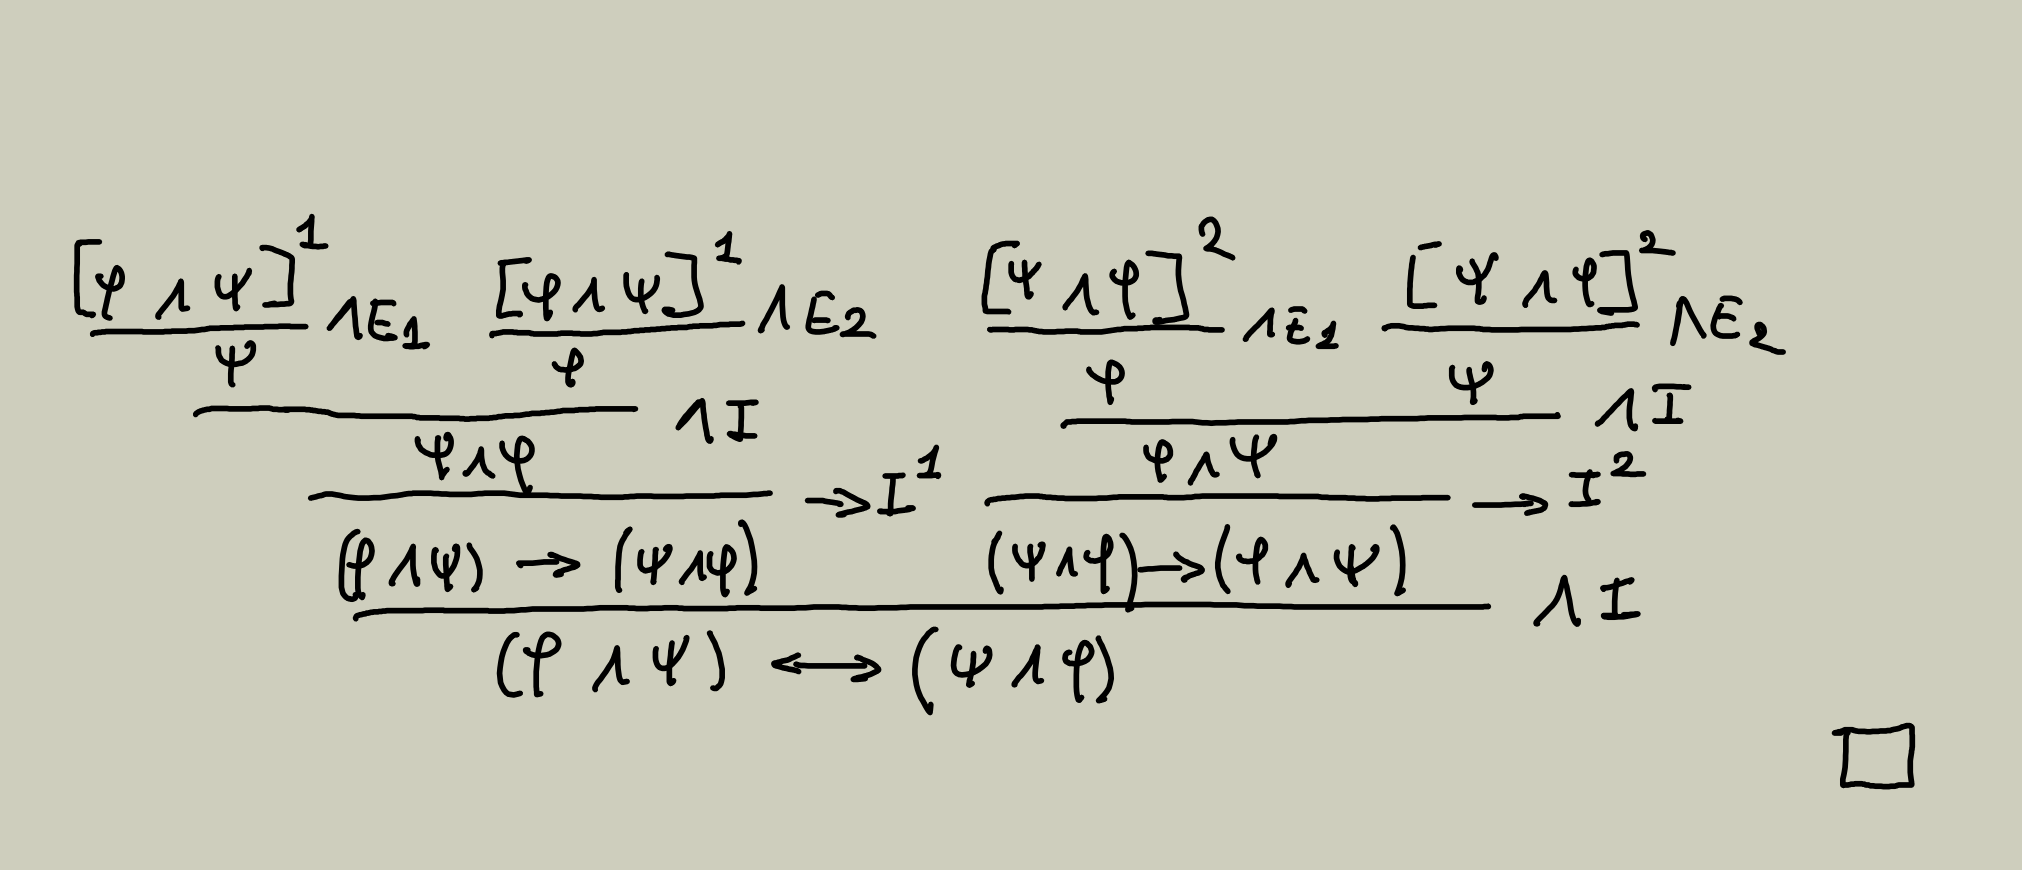
\includegraphics[width=13cm, height=5.6cm]{deriv1}
\end{center}
\newpage
\subsection{Definizione di derivazione}

L'insieme di tutte le derivazioni del sistema di ND$_p$ \`{e} il minimo insieme $X$ t.c.
\begin{itemize}
\item $\varphi \in X$ se $\varphi \in PROP$ (una formula atomica \`{e} una derivazione atomica).
\item Suponiamo di avere una derivaziione di $\varphi \in X$ e una derivazione di $\psi \in X$, posso derivare $\varphi \wedge \psi$:
\begin{center}
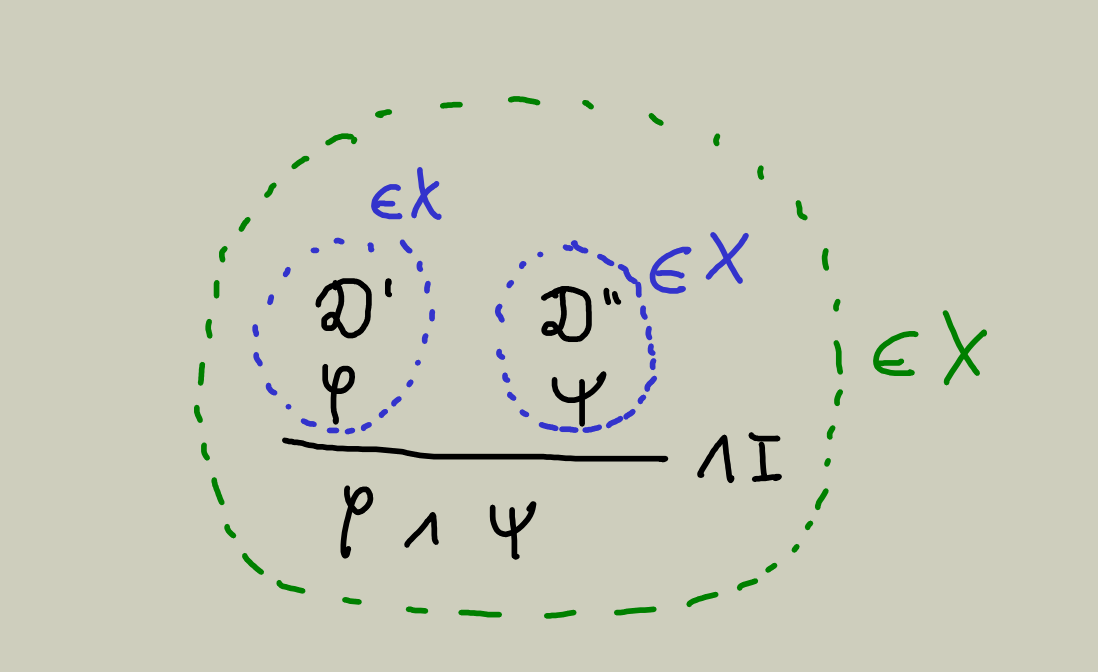
\includegraphics[width=10cm, height=5cm]{def1}
\end{center}
\item Supponiamo di avere una derivazione di $(\varphi \wedge \psi) \in X$ allora possiamo derivare $\varphi$ e $\psi$:
\begin{center}
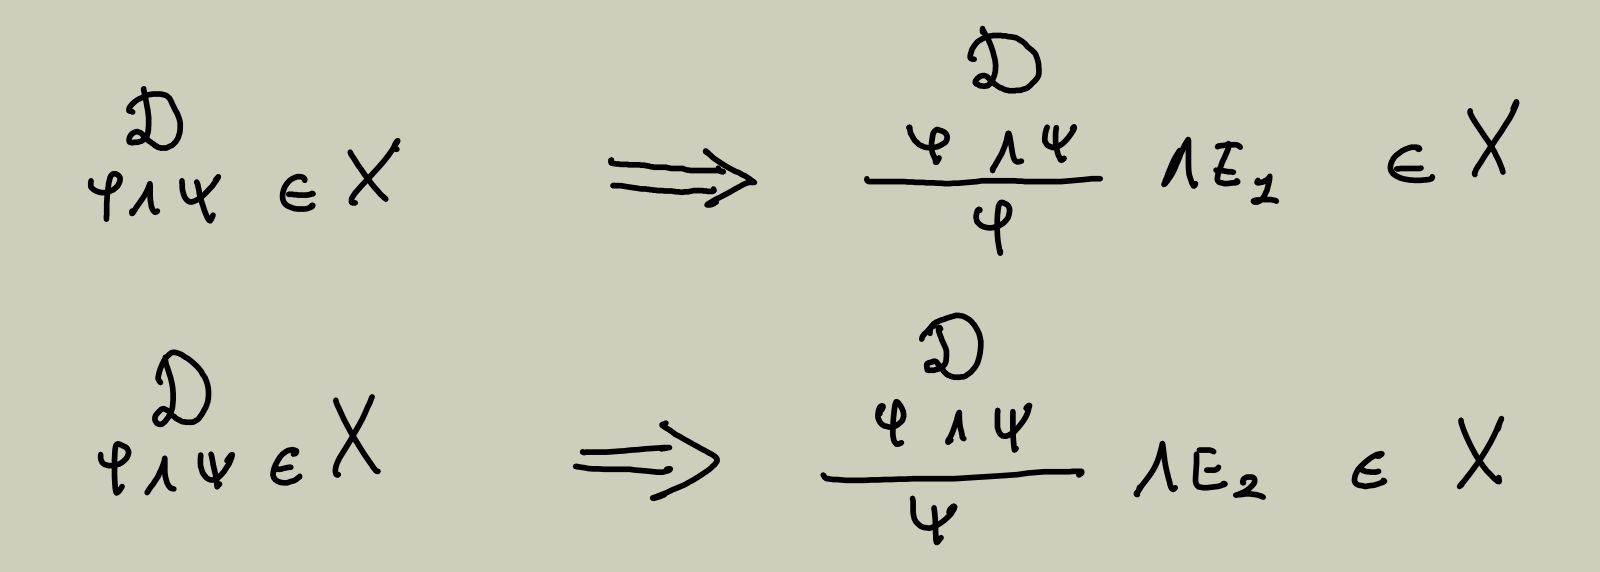
\includegraphics[width=10cm, height=4cm]{def2}
\end{center}
\item Supponiamo di avere una derivazione di $\varphi \in X$ e una derivazione di $(\varphi \to \psi) \in X$ allora possiamo derivare $\psi$:
\begin{center}
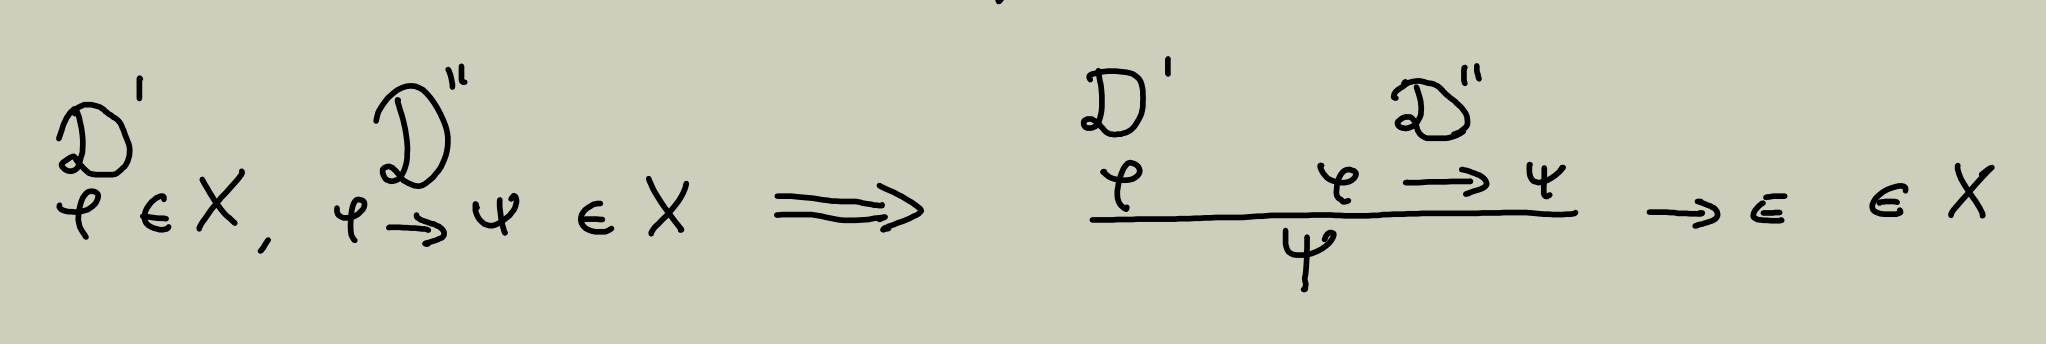
\includegraphics[width=13cm, height=3cm]{def3}
\end{center}
\end{itemize}






















\end{document}
